\documentclass[11pt]{article}
\usepackage[margin=0.75in]{geometry}
\usepackage{amsmath,amsfonts}
\usepackage{enumitem}
\usepackage{tikz}
\usepackage{pgfplots}
\usepackage{soul}

\usepackage{multicol}

\newcommand{\ds}{\displaystyle}
\newcommand{\N}{\mathbb{N}}
\newcommand{\R}{\mathbb{R}}
\newcommand{\C}{\mathbb{C}}
\newcommand{\re}{\operatorname{Re}}
\newcommand{\im}{\operatorname{Im}}
\newcommand{\on}{\operatorname}
\newcommand{\Log}{\on{Log}}
\newcommand{\Arg}{\on{Arg}}


\begin{document}
\newcounter{enumCount}
\pagestyle{empty}
\subsection*{Math 444 - Homework 9 \hfill Name: \underline{\hspace*{2in}}}

\begin{enumerate}
\item Let $\gamma(t) = 2e^{2it} - e^{it}$, $0 \le t \le 2\pi$. This path loops around the origin twice as shown below.  Calculate $\ds \int_\gamma \frac{dz}{z}$ for this path.  Hint: You can make it easier if you break the path into two simple closed curves, an inner one and an outer one, then apply the Cauchy Integral Formula. 
\begin{flushright}
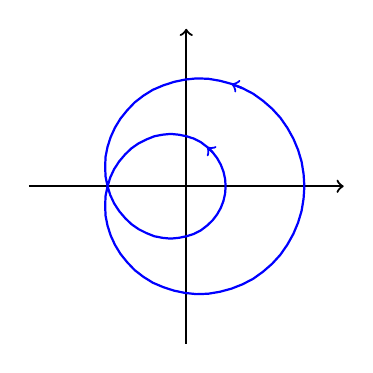
\begin{tikzpicture}[scale=0.5]
\draw[thick,->] (-4,0) -- (4,0);
\draw[thick,->] (0,-4) -- (0,4);
\draw[thick,blue] (1.0,0.0)--(0.986,0.188)--(0.945,0.372)--(0.877,0.549)--(0.784,0.715)--(0.667,0.867)--(0.528,1.0)--(0.37,1.12)--(0.195,1.21)--(0.00723,1.27)--(-0.191,1.31)--(-0.396,1.33)--(-0.603,1.31)--(-0.81,1.27)--(-1.01,1.19)--(-1.21,1.09)--(-1.39,0.965)--(-1.55,0.812)--(-1.7,0.636)--(-1.83,0.439)--(-1.93,0.225)--(-2.0,-0.00508)--(-2.05,-0.246)--(-2.06,-0.495)--(-2.05,-0.747)--(-2.0,-1.0)--(-1.92,-1.25)--(-1.81,-1.49)--(-1.67,-1.72)--(-1.5,-1.93)--(-1.31,-2.13)--(-1.09,-2.3)--(-0.849,-2.45)--(-0.59,-2.56)--(-0.316,-2.65)--(-0.0302,-2.71)--(0.263,-2.74)--(0.559,-2.73)--(0.855,-2.68)--(1.15,-2.6)--(1.43,-2.49)--(1.7,-2.35)--(1.95,-2.17)--(2.18,-1.97)--(2.39,-1.74)--(2.57,-1.48)--(2.72,-1.21)--(2.84,-0.924)--(2.93,-0.623)--(2.98,-0.313)--(3.0,-6.12e-16)--(2.98,0.313)--(2.93,0.623)--(2.84,0.924)--(2.72,1.21)--(2.57,1.48)--(2.39,1.74)--(2.18,1.97)--(1.95,2.17)--(1.7,2.35)--(1.43,2.49)--(1.15,2.6)--(0.855,2.68)--(0.559,2.73)--(0.263,2.74)--(-0.0302,2.71)--(-0.316,2.65)--(-0.59,2.56)--(-0.849,2.45)--(-1.09,2.3)--(-1.31,2.13)--(-1.5,1.93)--(-1.67,1.72)--(-1.81,1.49)--(-1.92,1.25)--(-2.0,1.0)--(-2.05,0.747)--(-2.06,0.495)--(-2.05,0.246)--(-2.0,0.00508)--(-1.93,-0.225)--(-1.83,-0.439)--(-1.7,-0.636)--(-1.55,-0.812)--(-1.39,-0.965)--(-1.21,-1.09)--(-1.01,-1.19)--(-0.81,-1.27)--(-0.603,-1.31)--(-0.396,-1.33)--(-0.191,-1.31)--(0.00723,-1.27)--(0.195,-1.21)--(0.37,-1.12)--(0.528,-1.0)--(0.667,-0.867)--(0.784,-0.715)--(0.877,-0.549)--(0.945,-0.372)--(0.986,-0.188)--cycle;
\draw[thick,->,blue] (0.667,0.867)--(0.528,1.0);
\draw[thick,->,blue] (1.43,2.49)--(1.15,2.6);
\end{tikzpicture}
\end{flushright}

\item Let $\gamma$ be the ellipse $|z-1|+|z-2| = 3$.  Use a partial fraction decomposition (i.e., find the constants $A$ and $B$ below) to calculate
$$\oint_\gamma \frac{z}{(z-1)(z-2)} \, dz = \oint_\gamma  \frac{A}{z-1} + \frac{B}{z-2} \, dz.$$
\begin{flushright}
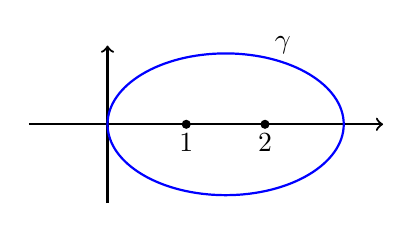
\begin{tikzpicture}[scale=1]
\draw[thick,->] (-1,0) -- (3.5,0);
\draw[thick,->] (0,-1) -- (0,1);
\filldraw (1,0) circle (0.05) node[below] {1};
\filldraw (2,0) circle (0.05) node[below] {2};
\draw[thick, blue,yscale=0.6] (1.5,0) circle (1.5);
\draw (2,1.0) node[right] {$\gamma$};
\end{tikzpicture}
\end{flushright}


\item What if you calculate the integral in problem 2 by splitting the elliptical path into a sum of two separate integrals along positively oriented paths $\gamma_1$ and $\gamma_2$ as shown in the figure below?  Find the values of $\ds \oint_{\gamma_1} \frac{z}{(z-1)(z-2)} \, dz$ and $\ds \oint_{\gamma_2} \frac{z}{(z-1)(z-2)} \, dz$.  Check to see if the sum of these two integrals is the same as the integral in problem 2. 
\begin{flushright}
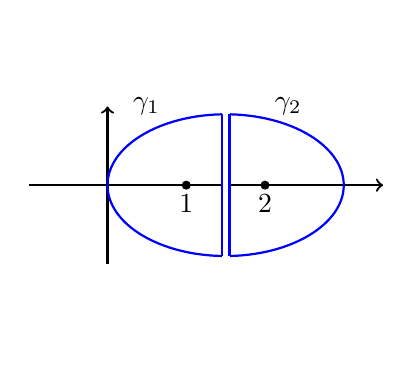
\begin{tikzpicture}[scale=1]
\draw[thick,->] (-1,0) -- (3.5,0);
\draw[thick,->] (0,-1) -- (0,1);
\filldraw (1,0) circle (0.05) node[below] {1};
\filldraw (2,0) circle (0.05) node[below] {2};
\draw[thick, blue,yscale=0.6] (1.5,0) circle (1.5);
\fill[white] (1.45,-2) rectangle (1.55,2);
\draw[thick, blue] (1.45,0.90) -- (1.45,-0.9);
\draw[thick, blue] (1.55,0.90) -- (1.55,-0.9);
\draw (2,1.0) node[right] {$\gamma_2$};
\draw (0.2,1.0) node[right] {$\gamma_1$};
\end{tikzpicture}
\end{flushright}


\item What is the power series for $f(z) = \dfrac{z}{z^2 - 2i}$ centered at $w = 0$?  What is the radius of convergence for that power series?  
\vfill

\setcounter{enumCount}{\theenumi}
\end{enumerate}

\newpage

\noindent 
\textit{Use Cauchy's integral formulas (including for derivatives) to evaluate the following.}
\begin{multicols}{3}
\begin{enumerate}
\setcounter{enumi}{\theenumCount}
\item $\ds \oint_{|z-3|=2} \frac{e^z}{z(z-3)} \, dz$
\item $\ds \oint_{|z| = 4} \frac{e^z}{z(z-3)} \, dz$
\item $\ds \oint_{|z| = 4} \frac{\exp(3z)}{(z-\pi i)^2} \, dz$
\setcounter{enumCount}{\theenumi}
\end{enumerate}
\end{multicols}
\vfill
\vfill 


%\item Calculate $\ds \oint_{|z|=2} \frac{e^z}{z^2+1} \, dz$.
%\vfill

%\item Suppose that $D$ is a simply connected region in $\C$ and $f$ and $g$ are both holomorphic on an open region containing $D$.  Let $\partial D$ denote the boundary of $D$ and assume it is piecewise smooth. If $f(z) = g(z)$ for all $z \in \partial D$, show that $f(z) = g(z)$ for all $z \in D$. 
%\vfill



%\item Let $p(z) = (z-\frac{1}{2})(z-2)(z-\frac{i}{2})$.  What is the winding number of the path $\gamma_1(t) = p(e^{it}), 0 \le t \le 2 \pi$ around the origin? What about the path $\gamma_2(t) = p(3e^{it}), 0 \le t \le 2\pi$? 
%\vfill
%
%\item What is the winding number of the path $\gamma(t)= 2e^{3it} + 5 e^{2it} - 3e^{it}$, $0 \le t \le 2\pi$ around the origin? Hint: $\gamma(t)$ is a polynomial function of $e^{it}$.  What are the roots of that polynomial?
%\vfill

\begin{multicols}{3}
\begin{enumerate}
\setcounter{enumi}{\theenumCount}
\item $\ds \oint_{|z| = 3} \Log(z-4i) \, dz$
\item $\ds \oint_{|z|=1} \frac{\cos(2z)}{z^3} \, dz$
\item $\ds \oint_{|z|=3} \frac{\exp(2z)}{(z-1)^2(z-2)} \, dz$
\setcounter{enumCount}{\theenumi}
\end{enumerate}
\end{multicols}
\vfill
\vfill


%\begin{multicols}{2}
%\begin{enumerate}
%\setcounter{enumi}{\theenumCount}
%\setcounter{enumCount}{\theenumi}
%\end{enumerate}
%\end{multicols}
%\vfill
%
%
%\begin{multicols}{2}
%\begin{enumerate}
%\setcounter{enumi}{\theenumCount}
%\item $\ds \left( \frac{\cos z}{z} \right)^2$
%\setcounter{enumCount}{\theenumi}
%\end{enumerate}
%\end{multicols}
%\vfill
%


\begin{enumerate}
\setcounter{enumi}{\theenumCount}


\item Let $p(z) = (z-\frac{1}{2})(z-2)(z-\frac{i}{2})$.  What is the winding number of the path $\gamma_1(t) = p(e^{it}), 0 \le t \le 2 \pi$ around the origin? What about the path $\gamma_2(t) = p(3e^{it}), 0 \le t \le 2\pi$? 
\vfill

\item What is the winding number of the path $\gamma(t)= 2e^{3it} + 5 e^{2it} - 3e^{it}$, $0 \le t \le 2\pi$ around the origin? Hint: $\gamma(t)$ is a polynomial function of $e^{it}$.  What are the roots of that polynomial?
\vfill

%\item If $p(z)$ is a polynomial with no roots on the unit circle, then prove that the integral of $\dfrac{1}{z}$ on the path $\gamma(t) = p(e^{i t})$ with $0 \le t \le 2 \pi$ is the same as $\ds \oint_C \frac{p'(z)}{p(z)} \, dz$ where $C$ is the unit circle.
%\vfill
%\vfill

\setcounter{enumCount}{\theenumi}
\end{enumerate}
%\begin{multicols}{2}
%\begin{enumerate}
%\setcounter{enumi}{\theenumCount}
%\item $\ds \frac{1}{(z+4)(z+1)^2}$
%\setcounter{enumCount}{\theenumi}
%\end{enumerate}
%\end{multicols}
%\vfill



\end{document}
